\chapter{Resultados e Análise Computacional} \label{ch:resultados}

\section{Instâncias e Ambiente de Testes}

Os experimentos computacionais foram conduzidos utilizando um conjunto de 42 instâncias de teste geradas sinteticamente, abrangendo diferentes cenários do Problema da Distribuição de Disciplinas (DPD). As instâncias variam em tamanho (62 a 214 disciplinas), número de professores (22 a 69), complexidade das restrições de carga horária e distribuição de preferências entre áreas de conhecimento.

Para cada experimento, foram selecionadas aleatoriamente 10 instâncias dentre as 42 disponíveis, garantindo representatividade estatística e mantendo o tempo total de experimentação viável. As mesmas instâncias foram utilizadas em todas as configurações testadas de um mesmo parâmetro, assegurando comparabilidade direta dos resultados.

Todas as execuções foram realizadas com limite de tempo global de 400 segundos por instância. O solver utilizado foi o SCIP 7.0 \cite{gamrath_2020_scip}, integrado com as heurísticas LNS e GRASP desenvolvidas neste trabalho. A calibração dos parâmetros da heurística LNS foi conduzida de forma incremental, conforme a abordagem \emph{one-factor-at-a-time}: primeiro determinou-se a melhor taxa de destruição, em seguida o melhor sentido de ordenação e, finalmente, o melhor limite de tempo para o sub-MIP. Essa estratégia permite isolar o efeito de cada parâmetro e identificar a configuração mais adequada de forma sistemática.

Para a seleção do melhor valor de cada parâmetro, adotou-se a seguinte hierarquia de critérios de desempate: (i)~tempo de execução, (ii)~gap de otimalidade e (iii)~número de nós restantes na árvore de Branch-and-Bound (\emph{nodes left}). Quando os critérios de maior prioridade apresentaram empate entre as configurações, o critério subsequente foi utilizado como desempate.

\section{Análise Interna das Configurações da LNS}

\subsection{Impacto da Taxa de Destruição (10\%, 25\%, 50\% e 75\%)}

A primeira análise experimental investigou o impacto da taxa de destruição (\texttt{lns\_perc}) na qualidade das soluções e no desempenho computacional. Foram testadas quatro configurações: 10\%, 25\%, 50\% e 75\% de destruição, mantendo fixos o tempo máximo do LNS (30s por chamada), a ordenação (crescente) e o tempo total de execução (400s).

% ============================================
% TABELAS - RESULTADOS DOS EXPERIMENTOS LNS
% ============================================

% Pacotes necessários: booktabs, multirow, array

% ============================================
% TABELA 1: Impacto da Taxa de Destruição - Tempo
% ============================================
\begin{table}[htbp]
\centering
\caption{Tempo de execução (segundos) para diferentes taxas de destruição do LNS. Configuração: ordenação crescente, tempo LNS = 30s, limite global = 400s.}
\label{tab:lns_cand_tempo}
\small
\begin{tabular}{@{}lrrrrrrrr@{}}
\toprule
\textbf{Instância} & \textbf{Disciplinas} & \textbf{Profs} & \textbf{Relax.} & \textbf{10\%} & \textbf{25\%} & \textbf{50\%} & \textbf{75\%} & \textbf{Melhor} \\
\midrule
input2  & 79  & 24 & 4,04    & 17,07  & 17,66  & 16,98  & 17,04  & Relax. \\
input5  & 84  & 29 & 113,03  & 145,27 & 145,04 & 145,71 & 143,63 & Relax. \\
input6  & 113 & 31 & 1,07    & 2,47   & 2,40   & 2,33   & 2,22   & Relax. \\
input7  & 99  & 28 & 400,02  & 400,02 & 400,02 & 400,02 & 400,02 & Empate \\
input9  & 133 & 41 & 17,06   & 72,52  & 72,33  & 72,57  & 73,48  & Relax. \\
input13 & 125 & 39 & 29,13   & 60,21  & 59,56  & 59,04  & 59,43  & Relax. \\
input19 & 114 & 39 & 2,11    & 1,39   & 1,44   & 1,42   & 1,47   & LNS 10\% \\
input20 & 113 & 40 & 0,95    & 4,69   & 4,56   & 4,59   & 5,02   & Relax. \\
input26 & 185 & 60 & 33,73   & 25,50  & 24,67  & 24,81  & 24,38  & LNS 75\% \\
input34 & 137 & 42 & 21,92   & 26,68  & 26,08  & 26,38  & 26,41  & Relax. \\
\midrule
\textbf{Média}  & 114 & 39 & 19,49 & 25,38 & 25,38 & 25,59 & 25,39 & Relax. \\
\textbf{Total}  & 1.296 & 412 & \textbf{623,05} & 755,82 & 753,76 & 753,84 & 753,10 & \textbf{Relax.} \\
\bottomrule
\end{tabular}
\end{table}

% ============================================
% TABELA 2: Impacto da Taxa de Destruição - Nodes Left
% ============================================
\begin{table}[htbp]
\centering
\caption{Número de nós restantes na árvore de Branch-and-Bound para diferentes taxas de destruição. Valores menores indicam maior progresso em direção à otimalidade.}
\label{tab:lns_cand_nodes}
\small
\begin{tabular}{@{}lrrrrrrrr@{}}
\toprule
\textbf{Instância} & \textbf{Disciplinas} & \textbf{Profs} & \textbf{Relax.} & \textbf{10\%} & \textbf{25\%} & \textbf{50\%} & \textbf{75\%} & \textbf{Melhor} \\
\midrule
input2  & 79  & 24 & 0      & 0      & 0      & 0      & 0      & -- \\
input5  & 84  & 29 & 0      & 0      & 0      & 0      & 0      & -- \\
input6  & 113 & 31 & 0      & 0      & 0      & 0      & 0      & -- \\
input7  & 99  & 28 & 66.230 & 62.628 & 60.540 & 61.056 & \textbf{58.921} & \textbf{75\%} \\
input9  & 133 & 41 & 0      & 0      & 0      & 0      & 0      & -- \\
input13 & 125 & 39 & 0      & 0      & 0      & 0      & 0      & -- \\
input19 & 114 & 39 & 0      & 0      & 0      & 0      & 0      & -- \\
input20 & 113 & 40 & 0      & 0      & 0      & 0      & 0      & -- \\
input26 & 185 & 60 & 0      & 0      & 0      & 0      & 0      & -- \\
input34 & 137 & 42 & 0      & 0      & 0      & 0      & 0      & -- \\
\midrule
\textbf{Média}  & 114 & 39 & 6.623 & 6.263 & 6.054 & 6.106 & 5.892 & LNS 75\% \\
\textbf{Total}  & 1.296 & 412 & 66.230 & 62.628 & 60.540 & 61.056 & \textbf{58.921} & \textbf{LNS 75\%} \\
\bottomrule
\end{tabular}
\end{table}

% ============================================
% TABELA 3: Impacto da Ordenação - Tempo
% ============================================
\begin{table}[htbp]
\centering
\caption{Tempo de execução (segundos) comparando ordenação crescente e decrescente. Configuração: 75\% de destruição, tempo LNS = 30s, limite global = 400s.}
\label{tab:lns_order_tempo}
\small
\begin{tabular}{@{}lrrrrrr@{}}
\toprule
\textbf{Instância} & \textbf{Disciplinas} & \textbf{Profs} & \textbf{Relax.} & \textbf{Crescente} & \textbf{Decrescente} & \textbf{Melhor} \\
\midrule
input4  & 123 & 46 & 400,05 & 400,04 & 400,05 & Crescente \\
input5  & 214 & 69 & 114,18 & 140,64 & 141,47 & Crescente \\
input12 & 115 & 37 & 5,79   & 25,70  & 25,84  & Crescente \\
input15 & 94  & 30 & 400,03 & 400,02 & 400,02 & Decrescente \\
input16 & 89  & 28 & 3,07   & 0,72   & 0,72   & Decrescente \\
input17 & 108 & 38 & 400,04 & 400,04 & 400,03 & Decrescente \\
input20 & 104 & 37 & 0,90   & 4,40   & 4,32   & Decrescente \\
input33 & 104 & 36 & 400,03 & 400,03 & 400,03 & Decrescente \\
input37 & 152 & 53 & 68,00  & 31,61  & 31,62  & Crescente \\
input38 & 62  & 22 & 0,16   & 0,28   & 0,28   & Decrescente \\
\midrule
\textbf{Média}  & 106 & 37 & 91,09 & 180,31 & 180,38 & Crescente \\
\textbf{Total}  & 1.271 & 433 & \textbf{1.792,24} & 1.803,48 & 1.804,48 & \textbf{Relax.} \\
\bottomrule
\end{tabular}
\end{table}

% ============================================
% TABELA 4: Impacto da Ordenação - Nodes Left
% ============================================
\begin{table}[htbp]
\centering
\caption{Número de nós restantes comparando ordenação crescente e decrescente.}
\label{tab:lns_order_nodes}
\small
\begin{tabular}{@{}lrrrrrr@{}}
\toprule
\textbf{Instância} & \textbf{Disciplinas} & \textbf{Profs} & \textbf{Relax.} & \textbf{Crescente} & \textbf{Decrescente} & \textbf{Melhor} \\
\midrule
input4  & 123 & 46 & 19.797 & 19.541 & 19.507 & Decrescente \\
input5  & 214 & 69 & 0      & 0      & 0      & -- \\
input12 & 115 & 37 & 0      & 0      & 0      & -- \\
input15 & 94  & 30 & 64.711 & \textbf{61.546} & 62.452 & \textbf{Crescente} \\
input16 & 89  & 28 & 0      & 0      & 0      & -- \\
input17 & 108 & 38 & 4.673  & 4.667  & 4.652  & Decrescente \\
input20 & 104 & 37 & 0      & 0      & 0      & -- \\
input33 & 104 & 36 & 50.279 & \textbf{46.243} & 47.063 & \textbf{Crescente} \\
input37 & 152 & 53 & 0      & 0      & 0      & -- \\
input38 & 62  & 22 & 0      & 0      & 0      & -- \\
\midrule
\textbf{Média}  & 106 & 37 & 13.946 & 13.200 & 13.367 & Crescente \\
\textbf{Total}  & 1.271 & 433 & 139.460 & \textbf{131.997} & 133.674 & \textbf{Crescente} \\
\bottomrule
\end{tabular}
\end{table}

% ============================================
% TABELA 5: Impacto do Tempo Máximo LNS - Tempo
% ============================================
\begin{table}[htbp]
\centering
\caption{Tempo de execução (segundos) para diferentes limites de tempo do sub-MIP. Configuração: 75\% de destruição, ordenação crescente, limite global = 400s.}
\label{tab:lns_time_tempo}
\small
\begin{tabular}{@{}lrrrrrrrrr@{}}
\toprule
\textbf{Inst.} & \textbf{Disc.} & \textbf{Prof.} & \textbf{Relax.} & \textbf{10s} & \textbf{50s} & \textbf{100s} & \textbf{200s} & \textbf{Melhor} \\
\midrule
input6  & 79  & 24 & 1,19   & 2,40   & 2,14   & 2,15   & \textbf{2,14}   & \textbf{200s} \\
input14 & 99  & 28 & 14,21  & 22,31  & 68,47  & 118,44 & 168,12 & Relax. \\
input15 & 94  & 30 & 400,03 & 400,02 & 400,02 & \textbf{76,31} & 77,09 & \textbf{100s} \\
input21 & 104 & 31 & 6,98   & \textbf{3,02}   & 3,04   & 3,05   & 3,10   & \textbf{10s} \\
input22 & 133 & 41 & 400,05 & 400,04 & 400,04 & 400,04 & 400,04 & 10s \\
input23 & 118 & 35 & 1,55   & \textbf{11,41} & 12,80  & 12,66  & 12,50  & \textbf{10s} \\
input27 & 125 & 39 & 4,93   & 7,45   & 7,34   & 7,33   & \textbf{7,31}   & \textbf{200s} \\
input29 & 103 & 39 & 400,03 & 400,03 & 19,42  & 19,40  & \textbf{19,39}  & \textbf{200s} \\
input33 & 104 & 36 & 400,03 & 400,03 & 400,03 & 400,03 & 400,03 & 200s \\
input38 & 62  & 22 & 0,16   & 0,28   & 0,28   & \textbf{0,28}   & 0,28   & \textbf{100s} \\
\midrule
\textbf{Média} & 104 & 33 & 162,92 & 164,77 & 162,11 & 160,27 & \textbf{159,46} & \textbf{200s} \\
\textbf{Total} & 1.125 & 358 & 1.629,16 & 1.647,01 & 1.313,60 & \textbf{1.039,68} & 1.090,00 & \textbf{100s} \\
\bottomrule
\end{tabular}
\end{table}

% ============================================
% TABELA 6: Impacto do Tempo Máximo LNS - Nodes Left
% ============================================
\begin{table}[htbp]
\centering
\caption{Número de nós restantes para diferentes limites de tempo do sub-MIP.}
\label{tab:lns_time_nodes}
\small
\begin{tabular}{@{}lrrrrrrrrr@{}}
\toprule
\textbf{Inst.} & \textbf{Disc.} & \textbf{Prof.} & \textbf{Relax.} & \textbf{10s} & \textbf{50s} & \textbf{100s} & \textbf{200s} & \textbf{Melhor} \\
\midrule
input6  & 79  & 24 & 0      & 0      & 0      & 0      & 0      & -- \\
input14 & 99  & 28 & 0      & 0      & 0      & 0      & 0      & -- \\
input15 & 94  & 30 & 54.355 & 63.056 & 59.819 & \textbf{0} & \textbf{0} & \textbf{100s} \\
input21 & 104 & 31 & 0      & 0      & 0      & 0      & 0      & -- \\
input22 & 133 & 41 & 21.528 & 29.161 & \textbf{25.100} & 50.411 & 33.000 & \textbf{50s} \\
input23 & 118 & 35 & 0      & 0      & 0      & 0      & 0      & -- \\
input27 & 125 & 39 & 0      & 0      & 0      & 0      & 0      & -- \\
input29 & 103 & 39 & 12.643 & 4.347  & \textbf{0} & \textbf{0} & \textbf{0} & \textbf{50s} \\
input33 & 104 & 36 & 47.460 & 48.110 & 45.505 & 1.524  & \textbf{539} & \textbf{200s} \\
input38 & 62  & 22 & 0      & 0      & 0      & 0      & 0      & -- \\
\midrule
\textbf{Média} & 104 & 33 & 13.599 & 14.467 & 13.042 & 5.194 & \textbf{3.354} & \textbf{200s} \\
\textbf{Total} & 1.125 & 358 & 135.986 & 144.674 & 130.424 & 51.935 & \textbf{33.539} & \textbf{200s} \\
\bottomrule
\end{tabular}
\end{table}

% ============================================
% TABELA 7: Impacto da Taxa de Destruição - GAP
% ============================================
\begin{table}[htbp]
\centering
\caption{Gap de otimalidade (\%) para diferentes taxas de destruição. Gap igual a zero indica solução ótima.}
\label{tab:lns_cand_gap}
\small
\begin{tabular}{@{}lrrrrrrrr@{}}
\toprule
\textbf{Instância} & \textbf{Disciplinas} & \textbf{Profs} & \textbf{Relax.} & \textbf{10\%} & \textbf{25\%} & \textbf{50\%} & \textbf{75\%} & \textbf{Melhor} \\
\midrule
input2  & 79  & 24 & 0,00 & 0,00 & 0,00 & 0,00 & 0,00 & Empate \\
input5  & 84  & 29 & 0,00 & 0,00 & 0,00 & 0,00 & 0,00 & Empate \\
input6  & 113 & 31 & 0,00 & 0,00 & 0,00 & 0,00 & 0,00 & Empate \\
input7  & 99  & 28 & 0,60 & 0,60 & 0,60 & 0,60 & 0,60 & Empate \\
input9  & 133 & 41 & 0,00 & 0,00 & 0,00 & 0,00 & 0,00 & Empate \\
input13 & 125 & 39 & 0,00 & 0,00 & 0,00 & 0,00 & 0,00 & Empate \\
input19 & 114 & 39 & 0,00 & 0,00 & 0,00 & 0,00 & 0,00 & Empate \\
input20 & 113 & 40 & 0,00 & 0,00 & 0,00 & 0,00 & 0,00 & Empate \\
input26 & 185 & 60 & 0,00 & 0,00 & 0,00 & 0,00 & 0,00 & Empate \\
input34 & 137 & 42 & 0,00 & 0,00 & 0,00 & 0,00 & 0,00 & Empate \\
\midrule
\textbf{Média}  & 114 & 39 & 0,06 & 0,06 & 0,06 & 0,06 & 0,06 & Empate \\
\textbf{Total}  & 1.296 & 412 & 0,60 & 0,60 & 0,60 & 0,60 & 0,60 & \textbf{Empate} \\
\bottomrule
\end{tabular}
\end{table}

% ============================================
% TABELA 8: Impacto da Ordenação - GAP
% ============================================
\begin{table}[htbp]
\centering
\caption{Gap de otimalidade (\%) comparando ordenação crescente e decrescente.}
\label{tab:lns_order_gap}
\small
\begin{tabular}{@{}lrrrrrr@{}}
\toprule
\textbf{Instância} & \textbf{Disciplinas} & \textbf{Profs} & \textbf{Relax.} & \textbf{Crescente} & \textbf{Decrescente} & \textbf{Melhor} \\
\midrule
input4  & 123 & 46 & 0,20 & 0,20 & 0,20 & Empate \\
input5  & 214 & 69 & 0,00 & 0,00 & 0,00 & Empate \\
input12 & 115 & 37 & 0,00 & 0,00 & 0,00 & Empate \\
input15 & 94  & 30 & 0,73 & 0,73 & 0,73 & Empate \\
input16 & 89  & 28 & 0,00 & 0,00 & 0,00 & Empate \\
input17 & 108 & 38 & 0,20 & 0,20 & 0,20 & Empate \\
input20 & 104 & 37 & 0,00 & 0,00 & 0,00 & Empate \\
input33 & 104 & 36 & 0,49 & 0,49 & 0,49 & Empate \\
input37 & 152 & 53 & 0,00 & 0,00 & 0,00 & Empate \\
input38 & 62  & 22 & 0,00 & 0,00 & 0,00 & Empate \\
\midrule
\textbf{Média}  & 106 & 37 & 0,16 & 0,16 & 0,16 & Empate \\
\textbf{Total}  & 1.271 & 433 & 1,62 & 1,62 & 1,62 & \textbf{Empate} \\
\bottomrule
\end{tabular}
\end{table}

% ============================================
% TABELA 9: Impacto do Tempo Máximo LNS - GAP
% ============================================
\begin{table}[htbp]
\centering
\caption{Gap de otimalidade (\%) para diferentes limites de tempo do sub-MIP.}
\label{tab:lns_time_gap}
\small
\begin{tabular}{@{}lrrrrrrrrr@{}}
\toprule
\textbf{Inst.} & \textbf{Disc.} & \textbf{Prof.} & \textbf{Relax.} & \textbf{10s} & \textbf{50s} & \textbf{100s} & \textbf{200s} & \textbf{Melhor} \\
\midrule
input6  & 79  & 24 & 0,00 & 0,00 & 0,00 & 0,00 & 0,00 & Empate \\
input14 & 99  & 28 & 0,00 & 0,00 & 0,00 & 0,00 & 0,00 & Empate \\
input15 & 94  & 30 & 0,73 & 0,73 & 0,73 & \textbf{0,00} & \textbf{0,00} & \textbf{100s} \\
input21 & 104 & 31 & 0,00 & 0,00 & 0,00 & 0,00 & 0,00 & Empate \\
input22 & 133 & 41 & 0,32 & 0,32 & 0,32 & 0,48 & 0,48 & Relax. \\
input23 & 118 & 35 & 0,00 & 0,00 & 0,00 & 0,00 & 0,00 & Empate \\
input27 & 125 & 39 & 0,00 & 0,00 & 0,00 & 0,00 & 0,00 & Empate \\
input29 & 103 & 39 & 0,19 & 0,19 & \textbf{0,00} & \textbf{0,00} & \textbf{0,00} & \textbf{50s} \\
input33 & 104 & 36 & 0,49 & 0,49 & 0,49 & \textbf{0,24} & \textbf{0,24} & \textbf{100s} \\
input38 & 62  & 22 & 0,00 & 0,00 & 0,00 & 0,00 & 0,00 & Empate \\
\midrule
\textbf{Média} & 104 & 33 & 0,17 & 0,17 & 0,15 & 0,07 & \textbf{0,07} & \textbf{100s} \\
\textbf{Total} & 1.125 & 358 & 1,73 & 1,73 & 1,54 & \textbf{0,72} & \textbf{0,72} & \textbf{100s} \\
\bottomrule
\end{tabular}
\end{table}

% ============================================
% TABELA 10: Avaliação Geral - Tempo
% ============================================
\begin{table}[htbp]
\centering
\caption{Tempo de execução (segundos) comparando Relaxação, LNS, GRASP e GRASP|LNS. Configuração LNS: 75\% destruição, crescente, 200s. Configuração GRASP: max\_iter=1, alpha=0.8, local\_search=0.}
\label{tab:geral_tempo}
\small
\begin{tabular}{@{}lrrrrrr@{}}
\toprule
\textbf{Instância} & \textbf{Disciplinas} & \textbf{Profs} & \textbf{Relax.} & \textbf{LNS} & \textbf{GRASP} & \textbf{GRASP|LNS} \\
\midrule
input5  & 214 & 69 & 112,63 & \textbf{54,46}  & 400,12 & 83,09 \\
input11 & 100 & 31 & 1,54   & 2,59   & 3,90   & \textbf{0,83} \\
input15 & 94  & 30 & 400,03 & \textbf{79,90}  & 400,02 & 400,02 \\
input16 & 89  & 28 & 3,07   & 0,75   & 8,38   & \textbf{0,36} \\
input19 & 95  & 29 & 2,03   & \textbf{1,45}   & 5,74   & 2,73 \\
input21 & 104 & 31 & 5,93   & \textbf{3,16}   & 13,45  & 4,42 \\
input25 & 107 & 34 & 15,63  & \textbf{9,27}   & 37,64  & 9,54 \\
input30 & 109 & 36 & 3,21   & \textbf{1,36}   & 7,94   & 2,36 \\
input35 & 169 & 53 & 186,72 & \textbf{63,27}  & 400,07 & 71,20 \\
input42 & 142 & 35 & \textbf{6,91}   & 8,18   & 20,19  & 13,39 \\
\midrule
\textbf{Média} & 106 & 33 & 73,76 & \textbf{22,44} & 129,75 & 58,79 \\
\textbf{Total} & 1.329 & 409 & 744,13 & \textbf{230,05} & 1.314,27 & 594,92 \\
\bottomrule
\end{tabular}
\end{table}

% ============================================
% TABELA 11: Avaliação Geral - Nodes Left
% ============================================
\begin{table}[htbp]
\centering
\caption{Número de nós restantes comparando Relaxação, LNS, GRASP e GRASP|LNS.}
\label{tab:geral_nodes}
\small
\begin{tabular}{@{}lrrrrrr@{}}
\toprule
\textbf{Instância} & \textbf{Disciplinas} & \textbf{Profs} & \textbf{Relax.} & \textbf{LNS} & \textbf{GRASP} & \textbf{GRASP|LNS} \\
\midrule
input5  & 214 & 69 & 0      & \textbf{0}      & 8.037  & \textbf{0} \\
input11 & 100 & 31 & 0      & \textbf{0}      & 0      & \textbf{0} \\
input15 & 94  & 30 & 64.364 & \textbf{0}      & 7.526  & 2.324 \\
input16 & 89  & 28 & 0      & \textbf{0}      & 0      & \textbf{0} \\
input19 & 95  & 29 & 0      & \textbf{0}      & 0      & \textbf{0} \\
input21 & 104 & 31 & 0      & \textbf{0}      & 0      & \textbf{0} \\
input25 & 107 & 34 & 0      & \textbf{0}      & 0      & \textbf{0} \\
input30 & 109 & 36 & 0      & \textbf{0}      & 0      & \textbf{0} \\
input35 & 169 & 53 & 0      & \textbf{0}      & 20.740 & \textbf{0} \\
input42 & 142 & 35 & 0      & \textbf{0}      & 0      & \textbf{0} \\
\midrule
\textbf{Média} & 106 & 33 & 6.436 & \textbf{0} & 3.630 & 232 \\
\textbf{Total} & 1.329 & 409 & 64.364 & \textbf{0} & 36.303 & 2.324 \\
\bottomrule
\end{tabular}
\end{table}

% ============================================
% TABELA 12: Avaliação Geral - GAP
% ============================================
\begin{table}[htbp]
\centering
\caption{Gap de otimalidade (\%) comparando Relaxação, LNS, GRASP e GRASP|LNS.}
\label{tab:geral_gap}
\small
\begin{tabular}{@{}lrrrrrr@{}}
\toprule
\textbf{Instância} & \textbf{Disciplinas} & \textbf{Profs} & \textbf{Relax.} & \textbf{LNS} & \textbf{GRASP} & \textbf{GRASP|LNS} \\
\midrule
input5  & 214 & 69 & 0,00 & \textbf{0,00} & 1,01 & \textbf{0,00} \\
input11 & 100 & 31 & 0,00 & \textbf{0,00} & 0,00 & \textbf{0,00} \\
input15 & 94  & 30 & 0,73 & \textbf{0,00} & 0,24 & 0,24 \\
input16 & 89  & 28 & 0,00 & \textbf{0,00} & 0,00 & \textbf{0,00} \\
input19 & 95  & 29 & 0,00 & \textbf{0,00} & 0,00 & \textbf{0,00} \\
input21 & 104 & 31 & 0,00 & \textbf{0,00} & 0,00 & \textbf{0,00} \\
input25 & 107 & 34 & 0,00 & \textbf{0,00} & 0,00 & \textbf{0,00} \\
input30 & 109 & 36 & 0,00 & \textbf{0,00} & 0,00 & \textbf{0,00} \\
input35 & 169 & 53 & 0,00 & \textbf{0,00} & 2,21 & \textbf{0,00} \\
input42 & 142 & 35 & 0,00 & \textbf{0,00} & 0,00 & \textbf{0,00} \\
\midrule
\textbf{Média} & 106 & 33 & 0,07 & \textbf{0,00} & 0,35 & 0,02 \\
\textbf{Total} & 1.329 & 409 & 0,73 & \textbf{0,00} & 3,46 & 0,24 \\
\bottomrule
\end{tabular}
\end{table}


\textbf{Tempo de Execução.} A Tabela~\ref{tab:lns_cand_tempo} apresenta os tempos de execução para as 10 instâncias selecionadas. A configuração de relaxação (sem LNS) obteve o menor tempo médio, com 19,49 segundos, contra 25,39 segundos da melhor configuração LNS (75\%). Esse resultado é esperado, pois o \emph{overhead} introduzido pelas chamadas ao sub-MIP do LNS aumenta o tempo total, sobretudo em instâncias que já são resolvidas de forma ótima pelo Branch-and-Bound puro. Nove das dez instâncias foram resolvidas até a otimalidade por todas as configurações, e apenas a instância input7 atingiu o limite de tempo. Assim, o tempo de execução não foi suficiente para diferenciar as configurações LNS entre si.

\textbf{Gap de Otimalidade.} Em termos de gap, todas as configurações --- incluindo a relaxação --- apresentaram desempenho equivalente (0,60\% de gap total), com apenas a instância input7 permanecendo sem solução ótima comprovada (ver Tabela~\ref{tab:lns_cand_gap}). Esse empate impediu o uso do gap como critério de seleção.

\textbf{Nós Restantes (\emph{Nodes Left}).} Uma vez que tanto o tempo quanto o gap resultaram em empate, o critério de desempate utilizado foi a quantidade de nós restantes na árvore de Branch-and-Bound ao final da execução, métrica que reflete o progresso em direção à prova de otimalidade. A Tabela~\ref{tab:lns_cand_nodes} revela que a configuração com 75\% de destruição alcançou o menor total de nós restantes: \textbf{58.921 nós}, comparado a 66.230 (relaxação), 62.628 (10\%), 60.540 (25\%) e 61.056 (50\%). Todas as configurações obtiveram resultado idêntico em 9 das 10 instâncias (resolvidas até a otimalidade), mas na instância crítica input7, a taxa de 75\% demonstrou maior capacidade de exploração e poda da árvore. A Figura~\ref{fig:nodes_cand} apresenta visualmente a comparação dos totais, e a Figura~\ref{fig:avg_nodes_cand} exibe a média por instância, evidenciando a superioridade da configuração de 75\%.

% Gráfico: Taxa de Destruição - Nodes Left
\begin{figure}[htbp]
\centering
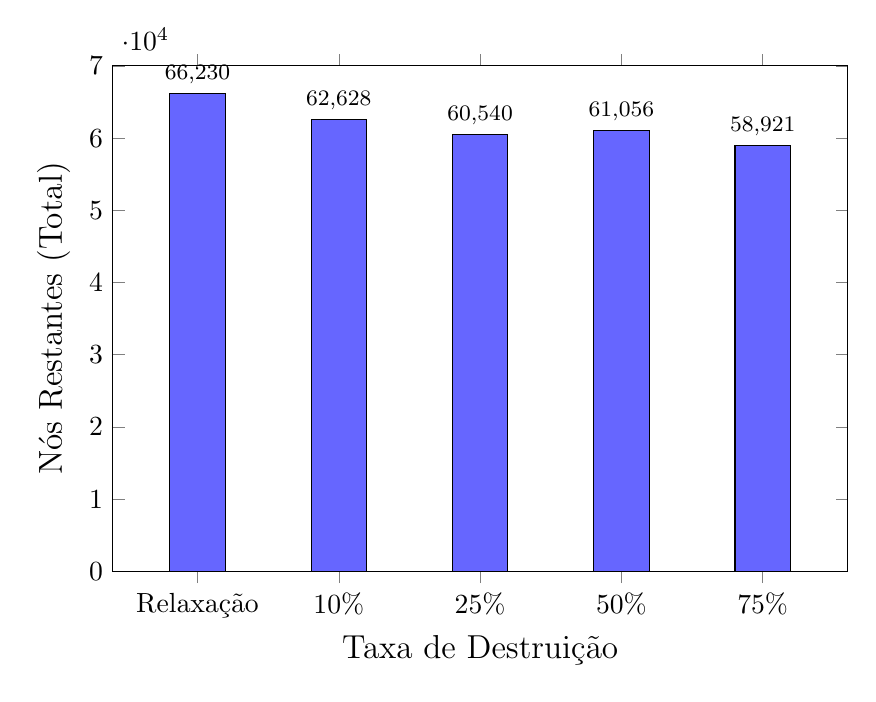
\begin{tikzpicture}
\begin{axis}[
    ybar,
    bar width=20pt,
    width=0.9\textwidth,
    height=8cm,
    ylabel={Nós Restantes (Total)},
    xlabel={Taxa de Destruição},
    symbolic x coords={Relaxação, 10\%, 25\%, 50\%, 75\%},
    xtick=data,
    nodes near coords,
    nodes near coords align={vertical},
    nodes near coords style={font=\footnotesize},
    ymin=0,
    ymax=70000,
    enlarge x limits=0.15,
    ylabel style={font=\large},
    xlabel style={font=\large},
    tick label style={font=\normalsize},
]
\addplot[fill=blue!60] coordinates {
    (Relaxação,66230)
    (10\%,62628)
    (25\%,60540)
    (50\%,61056)
    (75\%,58921)
};
\end{axis}
\end{tikzpicture}
\caption{Número total de nós restantes na árvore de Branch-and-Bound para diferentes taxas de destruição do LNS. A configuração de 75\% apresentou o melhor desempenho com 58.921 nós restantes.}
\label{fig:nodes_cand}
\end{figure}


% Gráfico: Taxa de Destruição - Média de Nós Restantes
\begin{figure}[htbp]
\centering
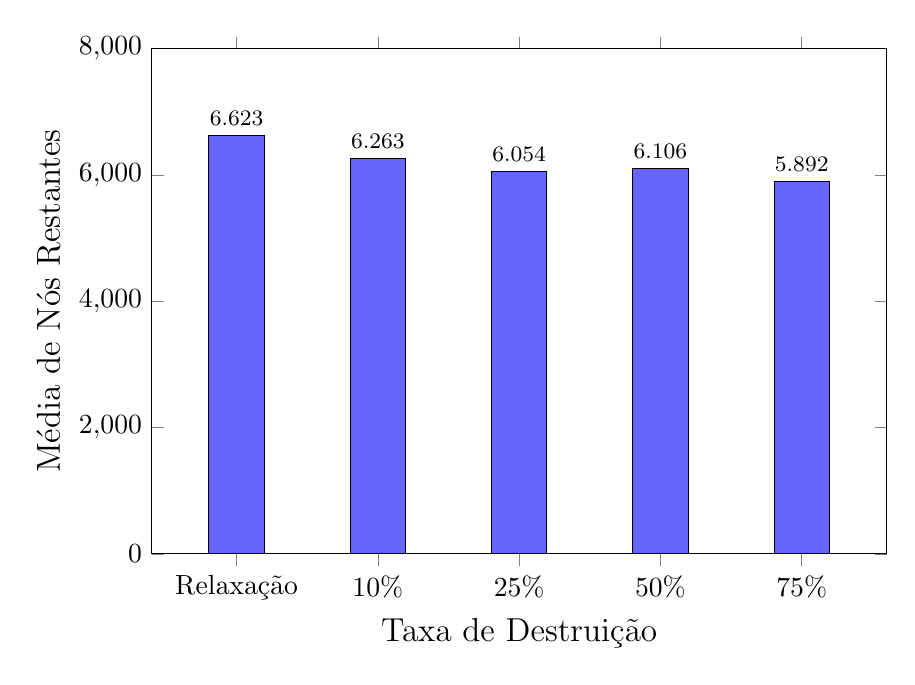
\begin{tikzpicture}
\begin{axis}[
    ybar,
    bar width=20pt,
    width=0.9\textwidth,
    height=8cm,
    ylabel={Média de Nós Restantes},
    xlabel={Taxa de Destruição},
    symbolic x coords={Relaxação, 10\%, 25\%, 50\%, 75\%},
    xtick=data,
    nodes near coords,
    nodes near coords align={vertical},
    nodes near coords style={font=\footnotesize},
    every node near coord/.append style={/pgf/number format/fixed,
        /pgf/number format/precision=0,
        /pgf/number format/use comma},
    ymin=0,
    ymax=8000,
    enlarge x limits=0.15,
    ylabel style={font=\large},
    xlabel style={font=\large},
    tick label style={font=\normalsize},
]
\addplot[fill=blue!60] coordinates {
    (Relaxação,6623)
    (10\%,6263)
    (25\%,6054)
    (50\%,6106)
    (75\%,5892)
};
\end{axis}
\end{tikzpicture}
\caption{Média de nós restantes na árvore de Branch-and-Bound para diferentes taxas de destruição do LNS. A configuração de 75\% apresentou a menor média, com 5.892 nós restantes por instância.}
\label{fig:avg_nodes_cand}
\end{figure}


\textbf{Conclusão Parcial.} A taxa de destruição de \textbf{75\%} foi selecionada para as análises subsequentes, pois demonstrou melhor capacidade de redução da árvore de busca na instância difícil. Esse resultado indica que vizinhanças maiores permitem ao LNS realizar explorações mais agressivas e produtivas do espaço de soluções, reforçando a estratégia de intensificação adotada pela matheurística.

\subsection{Impacto do Sentido de Ordenação (Crescente vs. Decrescente)}

Com a taxa de destruição fixada em 75\%, investigou-se o impacto do sentido de ordenação dos candidatos pelo valor de \texttt{avgPreferenceWeight}. Conforme descrito no Capítulo~\ref{ch:dpd}, a ordenação crescente prioriza a liberação de professores mais versáteis (maior número de preferências declaradas), enquanto a decrescente prioriza professores mais especializados (menor número de preferências).

\textbf{Tempo de Execução.} A Tabela~\ref{tab:lns_order_tempo} revela desempenho temporal praticamente idêntico entre as duas estratégias: 180,31 segundos (crescente) versus 180,38 segundos (decrescente) no tempo médio, com diferença inferior a 0,1 segundo. Das 10 instâncias testadas, quatro atingiram o limite de tempo em ambas as configurações (input4, input15, input17 e input33), e as demais apresentaram variações inferiores a 1 segundo. O tempo, portanto, não permitiu diferenciar as estratégias.

\textbf{Gap de Otimalidade.} Ambas as configurações mantiveram gap total idêntico de 1,62\%, distribuído entre quatro instâncias não resolvidas de forma ótima (input4, input15, input17 e input33), com gaps individuais variando de 0,20\% a 0,73\% (ver Tabela~\ref{tab:lns_order_gap}). O empate no gap impediu, novamente, seu uso como critério de seleção.

\textbf{Nós Restantes (\emph{Nodes Left}).} A métrica de nós restantes revelou vantagem para a ordenação crescente. A Tabela~\ref{tab:lns_order_nodes} mostra que a configuração crescente resultou em \textbf{131.997 nós restantes} no total, enquanto a decrescente deixou 133.674 nós --- uma redução de 1.677 nós (1,25\%). A diferença se concentra em duas instâncias críticas: input15 (61.546 vs.\ 62.452 nós) e input33 (46.243 vs.\ 47.063 nós). A Figura~\ref{fig:nodes_order} apresenta a comparação visual dos totais, e a Figura~\ref{fig:avg_nodes_order} exibe a média por instância.

% Gráfico: Ordenação - Nodes Left
\begin{figure}[htbp]
\centering
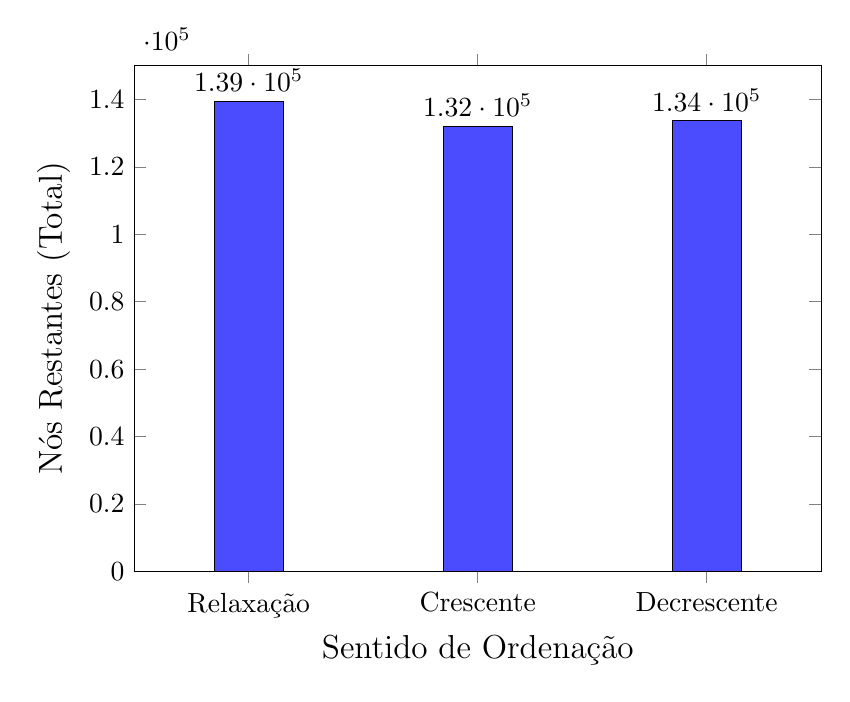
\begin{tikzpicture}
\begin{axis}[
    ybar,
    bar width=25pt,
    width=0.85\textwidth,
    height=8cm,
    ylabel={Nós Restantes (Total)},
    xlabel={Sentido de Ordenação},
    symbolic x coords={Relaxação, Crescente, Decrescente},
    xtick=data,
    nodes near coords,
    nodes near coords align={vertical},
    nodes near coords style={font=\normalsize},
    ymin=0,
    ymax=150000,
    enlarge x limits=0.25,
    ylabel style={font=\large},
    xlabel style={font=\large},
    tick label style={font=\normalsize},
]
\addplot[fill=blue!70] coordinates {
    (Relaxação,139460)
    (Crescente,131997)
    (Decrescente,133674)
};
\end{axis}
\end{tikzpicture}
\caption{Comparação do número total de nós restantes entre ordenação crescente e decrescente. A ordenação crescente (priorizando professores versáteis) obteve melhor desempenho com 131.997 nós restantes.}
\label{fig:nodes_order}
\end{figure}


% Gráfico: Ordenação - Média de Nós Restantes
\begin{figure}[htbp]
\centering
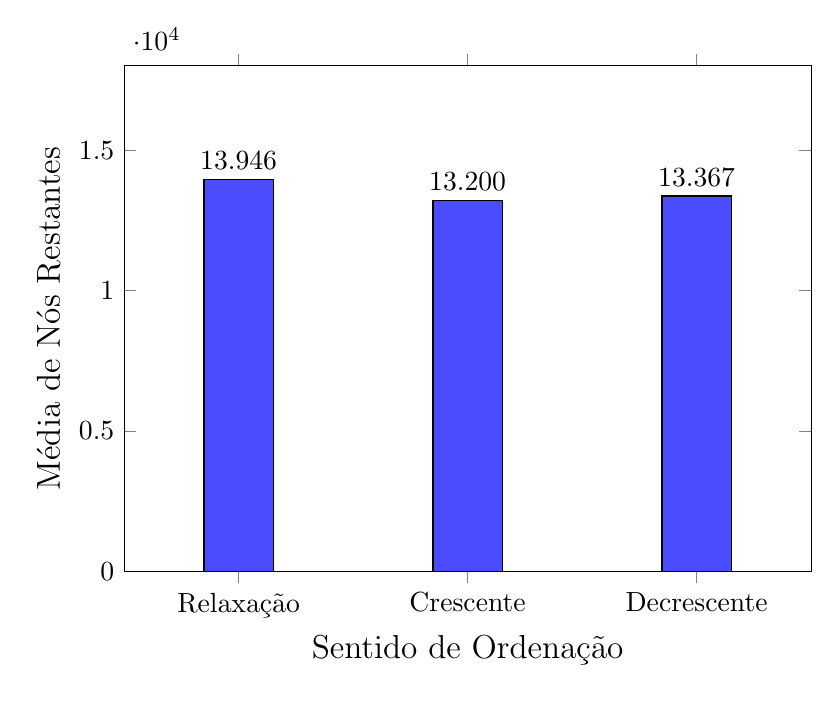
\begin{tikzpicture}
\begin{axis}[
    ybar,
    bar width=25pt,
    width=0.85\textwidth,
    height=8cm,
    ylabel={Média de Nós Restantes},
    xlabel={Sentido de Ordenação},
    symbolic x coords={Relaxação, Crescente, Decrescente},
    xtick=data,
    nodes near coords,
    nodes near coords align={vertical},
    nodes near coords style={font=\normalsize},
    every node near coord/.append style={/pgf/number format/fixed,
        /pgf/number format/precision=0,
        /pgf/number format/use comma},
    ymin=0,
    ymax=18000,
    enlarge x limits=0.25,
    ylabel style={font=\large},
    xlabel style={font=\large},
    tick label style={font=\normalsize},
]
\addplot[fill=blue!70] coordinates {
    (Relaxação,13946)
    (Crescente,13200)
    (Decrescente,13367)
};
\end{axis}
\end{tikzpicture}
\caption{Média de nós restantes por instância comparando ordenação crescente e decrescente. A ordenação crescente obteve a menor média, com 13.200 nós restantes.}
\label{fig:avg_nodes_order}
\end{figure}


\textbf{Interpretação.} A superioridade da ordenação \textbf{crescente} sugere que, para o DPD, priorizar a realocação de professores mais versáteis (generalistas) oferece maior flexibilidade para o sub-MIP encontrar rearranjos que melhorem a solução global. Professores generalistas possuem preferências por um maior número de disciplinas, o que amplia o espaço de busca do sub-MIP e facilita a satisfação simultânea de múltiplas restrições de carga horária. A ordenação crescente foi, portanto, adotada para as análises subsequentes.

\subsection{Impacto do Tempo Máximo do LNS (10s, 50s, 100s e 200s)}

Com os parâmetros de taxa de destruição (75\%) e ordenação (crescente) definidos, investigou-se o impacto do limite de tempo do sub-MIP (\texttt{lns\_time}). Foram testados quatro valores: 10s, 50s, 100s e 200s, mantendo o limite global de 400 segundos por instância.

\textbf{Tempo de Execução.} A Tabela~\ref{tab:lns_time_tempo} apresenta resultados contraintuitivos: embora se esperasse que limites maiores de LNS aumentassem o tempo total, observou-se comportamento não monotônico. O tempo médio foi de 164,77s (10s), 162,11s (50s), 160,27s (100s) e \textbf{159,46s (200s)}. O tempo total agregado reforça essa tendência: 1.629,16s (relaxação), 1.647,01s (10s), 1.313,60s (50s), \textbf{1.039,68s (100s)} e 1.090,00s (200s). Destaca-se a instância input15, em que as configurações de 100s e 200s resolveram o problema em $\sim$77s, contra 400s nas demais. Contudo, os resultados de tempo médio e tempo total apontam para configurações diferentes (200s e 100s, respectivamente), não permitindo uma conclusão unívoca por este critério.

Essa redução de tempo com limites maiores de LNS pode ser explicada pela capacidade de encontrar soluções de melhor qualidade mais cedo: uma incumbente mais forte permite podas mais agressivas na árvore de Branch-and-Bound, acelerando a convergência. Configurações com tempo insuficiente (10s) produzem melhorias marginais que não compensam o \emph{overhead} da heurística.

\textbf{Gap de Otimalidade.} A Tabela~\ref{tab:lns_time_gap} mostra que as configurações de 100s e 200s empataram com gap total de \textbf{0,72\%}, substancialmente inferior ao obtido pela relaxação e pelo LNS com 10s (ambos com 1,73\%). O destaque vai para a instância input15, resolvida até a otimalidade (gap 0,00\%) apenas pelas configurações de 100s e 200s, e para a instância input33, cujo gap caiu de 0,49\% (relaxação) para 0,24\% com 100s e 200s. Entretanto, o empate entre 100s e 200s impediu o uso do gap como critério final.

\textbf{Nós Restantes (\emph{Nodes Left}).} A Tabela~\ref{tab:lns_time_nodes} foi o critério de desempate definitivo. O total de nós restantes foi: 135.986 (relaxação), 144.674 (10s), 130.424 (50s), 51.935 (100s) e \textbf{33.539 (200s)}. A configuração de 200s reduziu os nós em 75,3\% em relação à relaxação e em 76,8\% em relação ao LNS com 10s. As instâncias input15 e input29 foram resolvidas completamente (0 nós restantes) pelas configurações de 100s e 200s, enquanto permaneceram com dezenas de milhares de nós nas configurações inferiores. Na instância input33, a configuração de 200s deixou apenas 539 nós, contra 1.524 com 100s. A Figura~\ref{fig:nodes_time} apresenta os totais, e a Figura~\ref{fig:avg_nodes_time} ilustra a média por instância, evidenciando a clara superioridade do limite de 200s.

% Gráfico: Tempo Máximo LNS - Nodes Left
\begin{figure}[htbp]
\centering
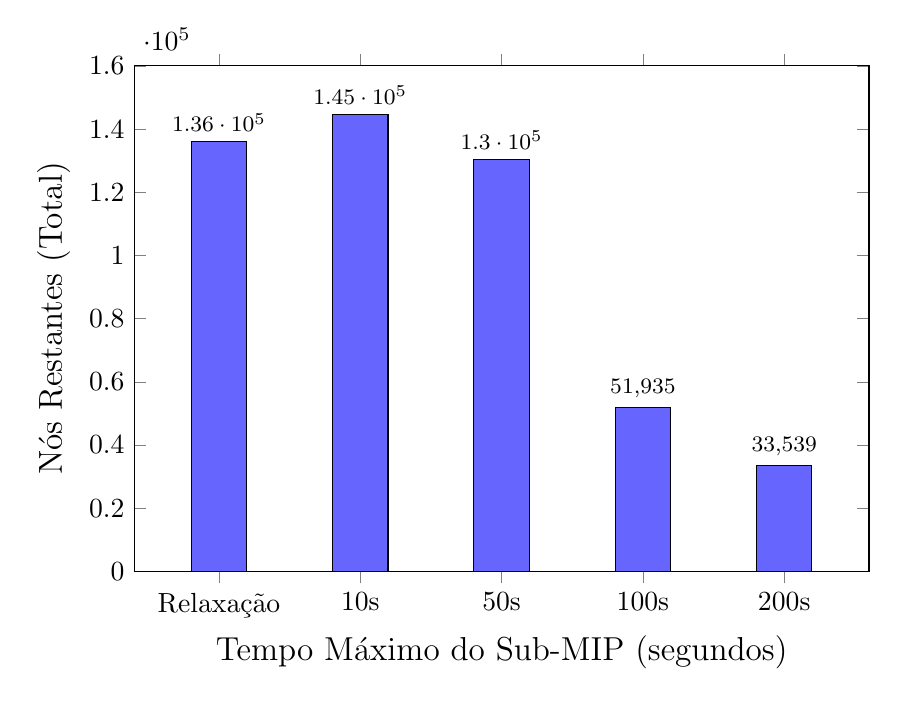
\begin{tikzpicture}
\begin{axis}[
    ybar,
    bar width=20pt,
    width=0.9\textwidth,
    height=8cm,
    ylabel={Nós Restantes (Total)},
    xlabel={Tempo Máximo do Sub-MIP (segundos)},
    symbolic x coords={Relaxação, 10s, 50s, 100s, 200s},
    xtick=data,
    nodes near coords,
    nodes near coords align={vertical},
    nodes near coords style={font=\footnotesize},
    ymin=0,
    ymax=160000,
    enlarge x limits=0.15,
    ylabel style={font=\large},
    xlabel style={font=\large},
    tick label style={font=\normalsize},
]
\addplot[fill=blue!60] coordinates {
    (Relaxação,135986)
    (10s,144674)
    (50s,130424)
    (100s,51935)
    (200s,33539)
};
\end{axis}
\end{tikzpicture}
\caption{Impacto do limite de tempo do sub-MIP no número de nós restantes. A configuração de 200s demonstrou o melhor desempenho com 33.539 nós, representando uma redução de 75,3\% em relação à relaxação pura.}
\label{fig:nodes_time}
\end{figure}


% Gráfico: Tempo Máximo LNS - Média de Nós Restantes
\begin{figure}[htbp]
\centering
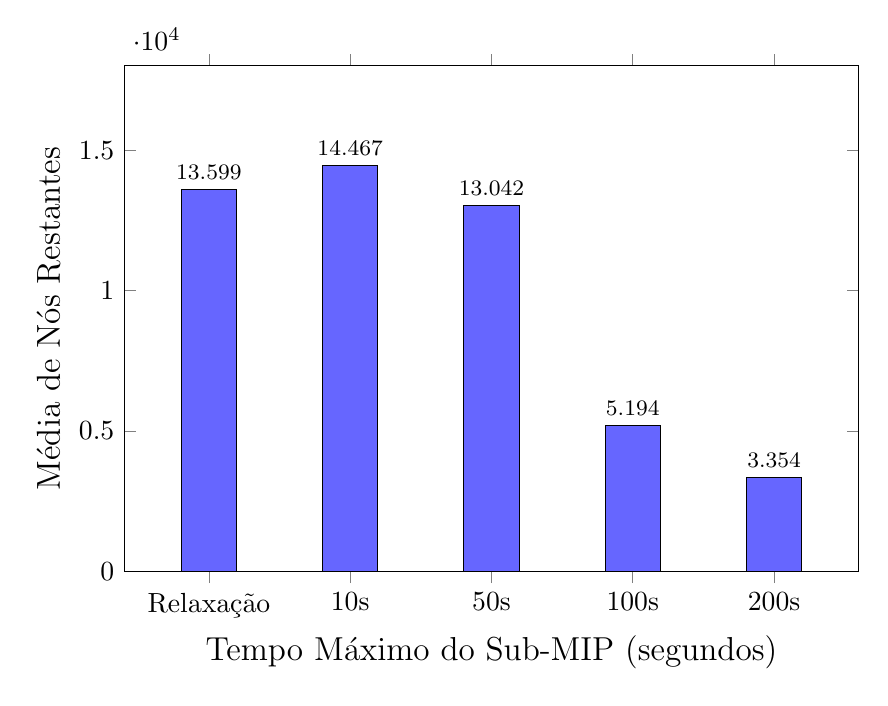
\begin{tikzpicture}
\begin{axis}[
    ybar,
    bar width=20pt,
    width=0.9\textwidth,
    height=8cm,
    ylabel={Média de Nós Restantes},
    xlabel={Tempo Máximo do Sub-MIP (segundos)},
    symbolic x coords={Relaxação, 10s, 50s, 100s, 200s},
    xtick=data,
    nodes near coords,
    nodes near coords align={vertical},
    nodes near coords style={font=\footnotesize},
    every node near coord/.append style={/pgf/number format/fixed,
        /pgf/number format/precision=0,
        /pgf/number format/use comma},
    ymin=0,
    ymax=18000,
    enlarge x limits=0.15,
    ylabel style={font=\large},
    xlabel style={font=\large},
    tick label style={font=\normalsize},
]
\addplot[fill=blue!60] coordinates {
    (Relaxação,13599)
    (10s,14467)
    (50s,13042)
    (100s,5194)
    (200s,3354)
};
\end{axis}
\end{tikzpicture}
\caption{Média de nós restantes por instância para diferentes limites de tempo do sub-MIP. A configuração de 200s alcançou a menor média, com 3.354 nós, representando uma redução de 75,3\% em relação à relaxação pura.}
\label{fig:avg_nodes_time}
\end{figure}


\textbf{Conclusão Parcial.} O limite de \textbf{200 segundos} demonstrou o melhor desempenho global, reduzindo drasticamente a árvore de busca e resolvendo instâncias que outras configurações não conseguiram. Para problemas combinatórios como o DPD, investir mais tempo em cada chamada do LNS é compensado por soluções de maior qualidade, que aceleram a convergência do Branch-and-Bound. O \emph{trade-off} entre intensidade (tempo por chamada) e frequência (número de chamadas) favorece claramente a intensidade para este problema.

\subsection{Resumo da Configuração Selecionada}

A Tabela~\ref{tab:config_final} resume os parâmetros selecionados ao longo da análise incremental.

\begin{table}[htbp]
\centering
\caption{Configuração final da heurística LNS selecionada pela análise incremental.}
\label{tab:config_final}
\small
\begin{tabular}{@{}llll@{}}
\toprule
\textbf{Parâmetro} & \textbf{Valores Testados} & \textbf{Selecionado} & \textbf{Critério Decisivo} \\
\midrule
Taxa de destruição (\texttt{lns\_perc}) & 10\%, 25\%, 50\%, 75\% & 75\% & Nós restantes \\
Ordenação (\texttt{lns\_order})         & Crescente, Decrescente  & Crescente & Nós restantes \\
Tempo do sub-MIP (\texttt{lns\_time})   & 10s, 50s, 100s, 200s   & 200s & Nós restantes \\
\bottomrule
\end{tabular}
\end{table}

Nota-se que, em todas as etapas, o tempo de execução e o gap de otimalidade não foram suficientes para diferenciar as configurações, sendo a métrica de nós restantes o critério de desempate definitivo. Esse padrão sugere que, para as instâncias avaliadas, o LNS atua predominantemente como acelerador da prova de otimalidade, reduzindo o esforço do Branch-and-Bound por meio de incumbentes de melhor qualidade.

\section{Comparativo de Desempenho: LNS, GRASP e Modelo Exato}

Com os parâmetros da LNS calibrados (75\% de destruição, ordenação crescente e tempo de sub-MIP de 200s), realizou-se um comparativo final entre quatro configurações: (i)~\textbf{Relaxação} (Branch-and-Bound puro, sem heurísticas primais customizadas), (ii)~\textbf{LNS} (apenas a heurística LNS proposta), (iii)~\textbf{GRASP} (apenas a heurística GRASP, com \texttt{max\_iter=1}, $\alpha=0{,}8$ e sem busca local \cite{jhonatan_grasp_dpd}) e (iv)~\textbf{GRASP|LNS} (ambas as heurísticas ativadas simultaneamente). As mesmas 10 instâncias foram utilizadas em todas as configurações.

\subsection{Análise do Tempo de Execução}

A Tabela~\ref{tab:geral_tempo} apresenta os tempos de execução para cada configuração. O \textbf{LNS} obteve o menor tempo médio: \textbf{22,44 segundos}, representando uma redução de 69,6\% em relação à relaxação (73,76s) e de 82,7\% em relação ao GRASP (129,75s). A configuração GRASP|LNS alcançou 58,79s de tempo médio, posicionando-se entre a relaxação e o LNS.

Dentre as 10 instâncias, o LNS foi o mais rápido em 7 delas, com destaque para a instância input15: enquanto a relaxação e o GRASP atingiram o limite de 400s, o LNS resolveu a instância em 79,90s. A instância input35, com 169 disciplinas e 53 professores, exemplifica o impacto da heurística: o LNS concluiu em 63,27s contra 186,72s da relaxação e 400,07s do GRASP. A Figura~\ref{fig:geral_tempo} ilustra a comparação dos tempos médios.

% Gráfico: Comparativo Geral - Tempo Médio
\begin{figure}[htbp]
\centering
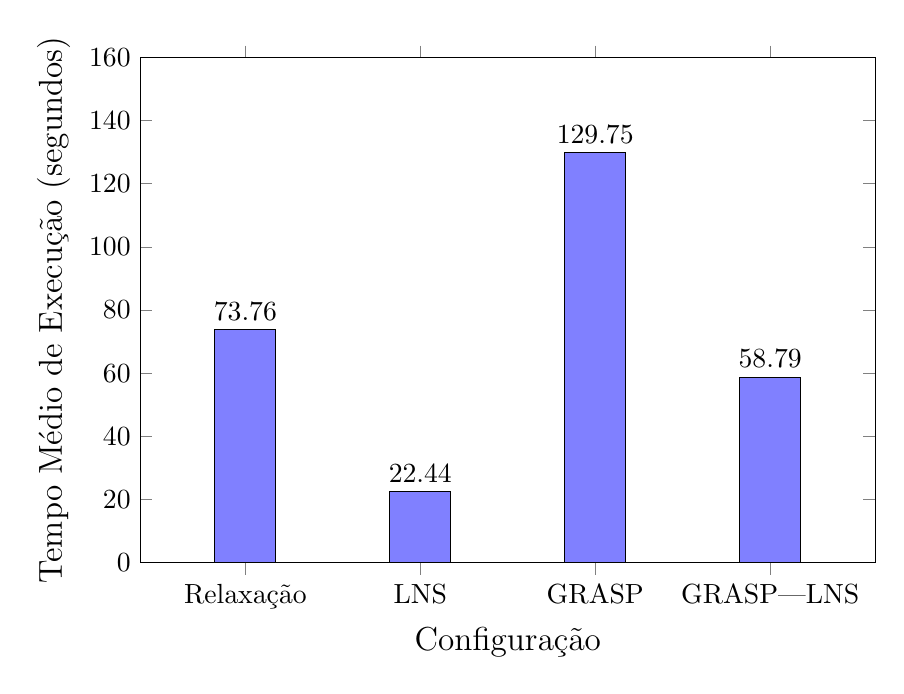
\begin{tikzpicture}
\begin{axis}[
    ybar,
    bar width=22pt,
    width=0.9\textwidth,
    height=8cm,
    ylabel={Tempo Médio de Execução (segundos)},
    xlabel={Configuração},
    symbolic x coords={Relaxação, LNS, GRASP, GRASP{|}LNS},
    xtick=data,
    nodes near coords,
    nodes near coords align={vertical},
    nodes near coords style={font=\normalsize, /pgf/number format/fixed,
        /pgf/number format/precision=2},
    ymin=0,
    ymax=160,
    enlarge x limits=0.2,
    ylabel style={font=\large},
    xlabel style={font=\large},
    tick label style={font=\normalsize},
]
\addplot[fill=blue!50] coordinates {
    (Relaxação,73.76)
    (LNS,22.44)
    (GRASP,129.75)
    (GRASP{|}LNS,58.79)
};
\end{axis}
\end{tikzpicture}
\caption{Tempo médio de execução (segundos) para cada configuração. O LNS obteve o menor tempo médio (22,44s), representando uma redução de 69,6\% em relação à relaxação pura e de 82,7\% em relação ao GRASP.}
\label{fig:geral_tempo}
\end{figure}


O GRASP apresentou o pior desempenho temporal, atingindo o limite de tempo em 3 das 10 instâncias (input5, input15 e input35). Esse resultado sugere que a heurística construtiva do GRASP, embora forneça soluções iniciais viáveis rapidamente, não contribui de forma eficaz para a redução da árvore de busca do Branch-and-Bound.

\subsection{Análise do Gap de Otimalidade}

A Tabela~\ref{tab:geral_gap} apresenta o gap de otimalidade para cada configuração. O \textbf{LNS} atingiu \textbf{gap total de 0,00\%}, provando a otimalidade de todas as 10 soluções encontradas. A relaxação obteve 0,73\% (devido à instância input15 não resolvida), a GRASP|LNS obteve 0,24\% (input15 com gap residual) e o GRASP apresentou o pior resultado com 3,46\% de gap total, com três instâncias sem solução ótima comprovada (input5 com 1,01\%, input15 com 0,24\% e input35 com 2,21\%). A Figura~\ref{fig:geral_gap} apresenta a comparação visual.

% Gráfico: Comparativo Geral - Gap de Otimalidade
\begin{figure}[htbp]
\centering
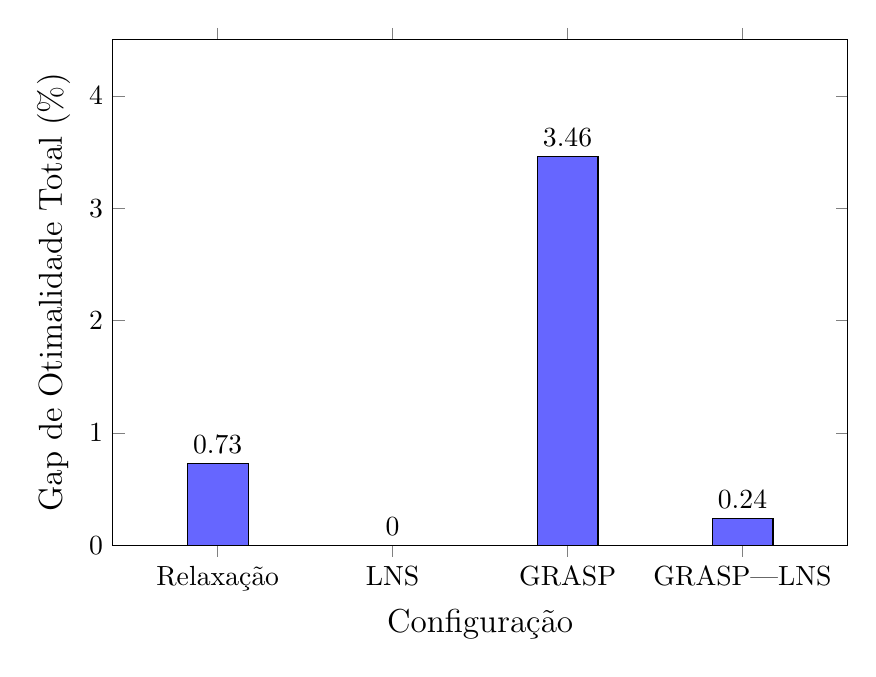
\begin{tikzpicture}
\begin{axis}[
    ybar,
    bar width=22pt,
    width=0.9\textwidth,
    height=8cm,
    ylabel={Gap de Otimalidade Total (\%)},
    xlabel={Configuração},
    symbolic x coords={Relaxação, LNS, GRASP, GRASP{|}LNS},
    xtick=data,
    nodes near coords,
    nodes near coords align={vertical},
    nodes near coords style={font=\normalsize, /pgf/number format/fixed,
        /pgf/number format/precision=2},
    ymin=0,
    ymax=4.5,
    enlarge x limits=0.2,
    ylabel style={font=\large},
    xlabel style={font=\large},
    tick label style={font=\normalsize},
]
\addplot[fill=blue!60] coordinates {
    (Relaxação,0.73)
    (LNS,0.00)
    (GRASP,3.46)
    (GRASP{|}LNS,0.24)
};
\end{axis}
\end{tikzpicture}
\caption{Gap de otimalidade total (\%) para cada configuração. O LNS atingiu gap zero, provando a otimalidade de todas as soluções encontradas.}
\label{fig:geral_gap}
\end{figure}


A superioridade do LNS no gap é particularmente expressiva: enquanto a relaxação pura não conseguiu provar a otimalidade da instância input15 em 400s, o LNS resolveu-a completamente. O GRASP, por sua vez, não apenas falhou em provar otimalidade, como também obteve soluções de pior qualidade em duas instâncias (input5 e input35), conforme indicado pelos gaps de 1,01\% e 2,21\%.

\subsection{Análise dos Nós Restantes}

A Tabela~\ref{tab:geral_nodes} confirma a superioridade do LNS. O \textbf{LNS alcançou 0 nós restantes} no total, indicando que todas as instâncias foram resolvidas até a otimalidade dentro do limite de tempo. A relaxação deixou 64.364 nós (todos da instância input15), o GRASP deixou 36.303 nós (distribuídos entre input5, input15 e input35) e a GRASP|LNS deixou 2.324 nós (apenas input15). A Figura~\ref{fig:geral_nodes} apresenta a comparação.

% Gráfico: Comparativo Geral - Nós Restantes (Total)
\begin{figure}[htbp]
\centering
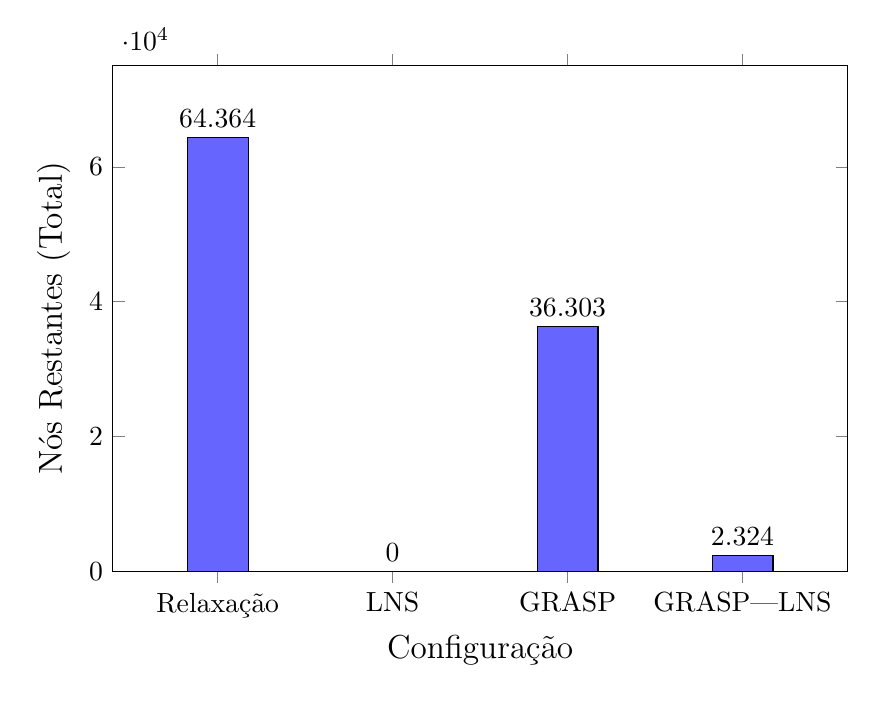
\begin{tikzpicture}
\begin{axis}[
    ybar,
    bar width=22pt,
    width=0.9\textwidth,
    height=8cm,
    ylabel={Nós Restantes (Total)},
    xlabel={Configuração},
    symbolic x coords={Relaxação, LNS, GRASP, GRASP{|}LNS},
    xtick=data,
    nodes near coords,
    nodes near coords align={vertical},
    nodes near coords style={font=\normalsize},
    every node near coord/.append style={/pgf/number format/fixed,
        /pgf/number format/precision=0,
        /pgf/number format/use comma},
    ymin=0,
    ymax=75000,
    enlarge x limits=0.2,
    ylabel style={font=\large},
    xlabel style={font=\large},
    tick label style={font=\normalsize},
]
\addplot[fill=blue!60] coordinates {
    (Relaxação,64364)
    (LNS,0)
    (GRASP,36303)
    (GRASP{|}LNS,2324)
};
\end{axis}
\end{tikzpicture}
\caption{Total de nós restantes na árvore de Branch-and-Bound para cada configuração. O LNS alcançou 0 nós restantes, resolvendo todas as instâncias até a otimalidade.}
\label{fig:geral_nodes}
\end{figure}


\subsection{Discussão dos Resultados}

Os resultados do comparativo evidenciam que a matheurística LNS proposta supera consistentemente tanto o Branch-and-Bound puro quanto o GRASP em todas as métricas avaliadas. A Tabela~\ref{tab:resumo_comparativo} sintetiza os principais indicadores.

\begin{table}[htbp]
\centering
\caption{Resumo comparativo das quatro configurações avaliadas.}
\label{tab:resumo_comparativo}
\small
\begin{tabular}{@{}lrrrr@{}}
\toprule
\textbf{Métrica} & \textbf{Relaxação} & \textbf{LNS} & \textbf{GRASP} & \textbf{GRASP|LNS} \\
\midrule
Tempo médio (s)        & 73,76  & \textbf{22,44} & 129,75 & 58,79 \\
Tempo total (s)        & 744,13 & \textbf{230,05} & 1.314,27 & 594,92 \\
Gap total (\%)         & 0,73   & \textbf{0,00}  & 3,46   & 0,24 \\
Nós restantes (total)  & 64.364 & \textbf{0}     & 36.303 & 2.324 \\
Instâncias ótimas      & 9/10   & \textbf{10/10} & 7/10   & 9/10 \\
\bottomrule
\end{tabular}
\end{table}

A análise revela três observações principais:

\begin{enumerate}
  \item \textbf{O LNS é o método mais eficaz.} Com a configuração calibrada (75\% de destruição, ordenação crescente, 200s de sub-MIP), o LNS resolveu todas as instâncias até a otimalidade, com tempo médio 3,3 vezes menor que a relaxação e 5,8 vezes menor que o GRASP. A estratégia de intensificação via sub-MIP gera incumbentes de alta qualidade que viabilizam podas mais eficientes na árvore de busca.

  \item \textbf{A combinação GRASP|LNS não supera o LNS isolado.} Embora a GRASP|LNS tenha apresentado desempenho superior à relaxação e ao GRASP, o \emph{overhead} da heurística construtiva GRASP não trouxe benefícios adicionais quando o LNS já estava ativo. Isso sugere que o LNS é capaz de encontrar incumbentes de qualidade suficiente sem a necessidade de uma solução inicial heurística dedicada.

  \item \textbf{O GRASP isolado apresenta limitações para o DPD.} O GRASP atingiu o limite de tempo em 30\% das instâncias e não conseguiu provar a otimalidade em 3 delas. A heurística construtiva, embora gere soluções viáveis rapidamente, não contribui de forma significativa para a redução do espaço de busca, e o \emph{overhead} computacional de sua execução a cada nó penaliza o desempenho global.
\end{enumerate}